% Masterclass Introduction: The Foundations of Trend Following
% Extracted from Algorithmic Trading Course (L5)

\section{Introduction: The Momentum Phenomenon}

\begin{frame}{Defining Momentum}
    \begin{definition}[A version of Momentum]
    In its most basic form: Find a moving average/trend.
        \begin{itemize}
        \item \textbf{Go Long} if 
            \begin{itemize}
            \item Level $>$ Moving average (+threshold)
            \item Short Moving Average $>$ Long Moving Average
            \item Trend is going up
            \end{itemize}
        \item \textbf{Go Short} if
            \begin{itemize}
            \item Level $<$ Moving average (-threshold)
            \item Short Moving Average $<$ Long Moving Average
            \item Trend is going down
            \end{itemize}
        \end{itemize}
    \end{definition}
\end{frame}

\begin{frame}{200 Years of Trend Following}
    \begin{figure}
    \centering
    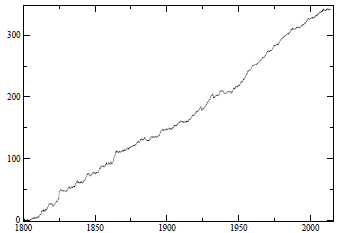
\includegraphics[scale=0.4]{docs/Figures/L5/Trend_Following_200y.png}
    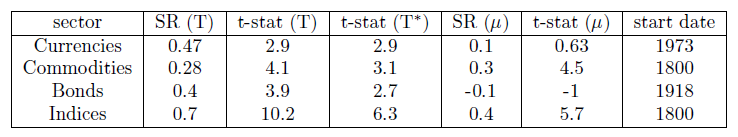
\includegraphics[scale=0.4]{docs/Figures/L5/Trend_Following_200y_table.png}
    \caption{Historical Performance of Trend Following (Lemp\'eri\`ere et al., 2014)}
    \end{figure}
    \textit{Insight:} A combined Sharpe Ratio of 0.72 over two centuries proves the persistence of this risk premium.
\end{frame}

\begin{frame}{Momentum Factoids: Why we trade it}
\begin{alertblock}{Desirable Properties}
    \begin{itemize}
    \item \textbf{Crisis Alpha:} Performs when volatility is high; acts as a form of insurance.
    \item \textbf{Positive Skewness:} Captures outsized wins while limiting frequent small losses.
    \item \textbf{Time Horizon Sensitivity:} Skewness appears greater when measured over longer horizons.
    \item \textbf{Straddle-like Payoff:} Empirically resembles the payoff of a long straddle.
    \end{itemize}
\end{alertblock}
\end{frame}

\begin{frame}{Taxonomy of Traditional Filtering}
\begin{alertblock}{Filtering Returns}
\begin{itemize}  
    \item Exponentially weighted moving averages (EWMA)
    \item Simple moving averages (SMA)
    \item Normalising and Winsorising signals
    \item \textbf{The Core Limit:} Levine and Pedersen (2015) show that in spite of the wide variety of models, momentum returns are often almost identical.
\end{itemize}
\end{alertblock}
\textit{Question:} How do we break this "identity trap"? \\
\textbf{Enter the Momentum Transformer.}
\end{frame}

\begin{frame}{Skewness by Horizon}
\begin{figure}
    \centering
    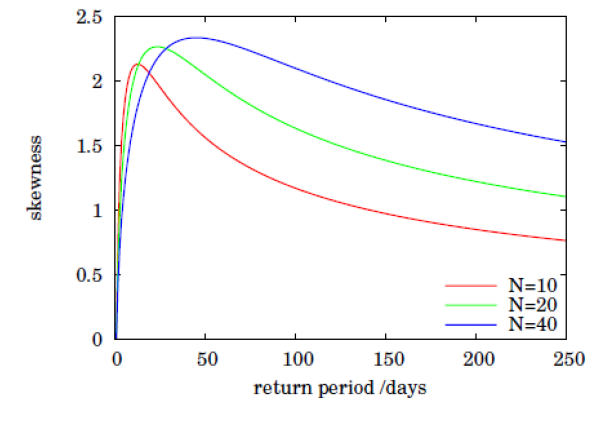
\includegraphics[width=0.45\textwidth]{docs/Figures/L5/MartinsSkewnessEWMA1.png}
    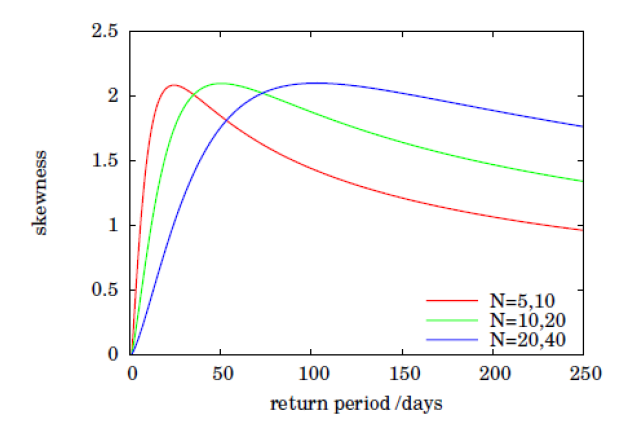
\includegraphics[width=0.45\textwidth]{docs/Figures/L5/MartinsSkewnessEWMA2.png}
    \caption{Skewness for various horizons (Martins-Zou)}
\end{figure}
We will use the Transformer to dynamically weight these horizons using Variable Selection Networks (VSN).
\end{frame}
